\clearpage
\subsection{Compound Statement} % (fold)
\label{sub:compound_statement}

\nameref{sub:branching} and \nameref{sub:looping} statements need to be able to include a number of instructions within their paths. Often languages will manage this by indicating that only a \emph{single} statement can be included in any of these paths, and then include the ability to code multiple statements in a \emph{single compound statement}.

\begin{figure}[h]
   \centering
   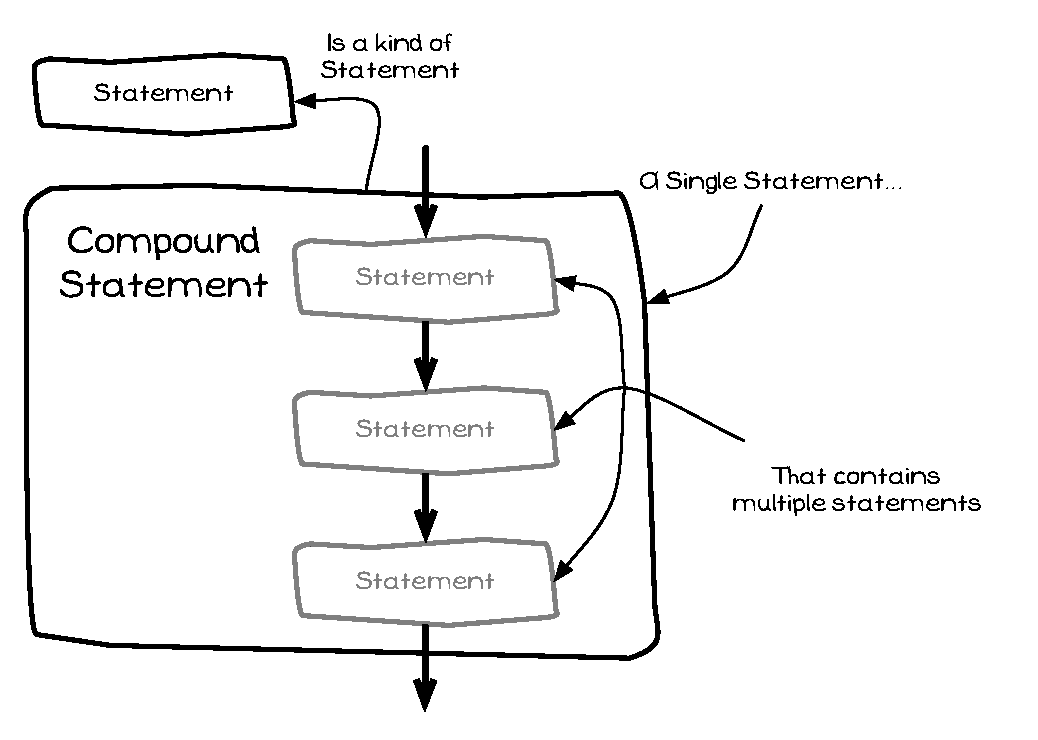
\includegraphics[width=\textwidth]{./topics/control-flow/diagrams/CompoundStatement} 
   \caption{A Compound Statement is a Statement that can contain other Statements}
   \label{fig:branching-compound-statement}
\end{figure}

\mynote{
\begin{itemize}
  \item A Compound Statement is a way of grouping \textbf{action}s, allowing you to create a single statement that contains multiple statements.
  \item Compound Statements are useful when combined with \nameref{sub:branching} and \nameref{sub:looping} Statements. Allowing you to put multiple statements within a path.
\end{itemize}
}

% subsection compound_statements (end)